\documentclass[a4paper,12pt]{article} % тип документа

% Поля страниц
\usepackage[left=2.5cm,right=2.5cm,top=1.5cm,bottom=2cm,bindingoffset=0cm]{geometry}
    
% Отступ после заголовка
\usepackage{indentfirst}

% Картинки
\usepackage{graphicx}
\graphicspath{{images/}}
\usepackage{placeins}

% Таблицы
\usepackage{booktabs}
% \usepackage{floatrow}
\usepackage{subcaption}

% Русский язык
\usepackage{cmap}  % поиск в PDF
\usepackage{mathtext}  % русские буквы в формулах
\usepackage[T2A]{fontenc}  % кодировка
\usepackage[utf8]{inputenc}  % кодировка исходного текста
\usepackage[english,russian]{babel}  % локализация и переносы

% Математика
\usepackage{amsmath}

% Ссылки TODO
% \usepackage[unicode=true]{hyperref}
% \usepackage[T1]{fontenc}

\begin{document}

\begin{center}   
\large{
Работа 2.1.3
\\\textbf{
Определение $C_p/C_v$ по скорости звука в газе
}}\\
\end{center}

\section{Аннотация}

\noindent\textbf{Цель работы:}
1) измерение частоты колебаний и длины волны при резонансе звуковых колебаний в газе, заполняющем трубу; 2) определение показателя адиабаты с помощью уравнения состояния идеального газа.

\smallskip
\noindent\textbf{В работе используются:}
звуковой генератор ГЗ; электронный осциллограф ЭО; микрофон; телефон; раздвижная труба; теплоизолированная труба, обогреваемая водой из термостата; баллон со сжатым углекислым газом; газгольдер.

\section{Теоретические сведения}
	
Скорость распространения звуковой волны в газах зависит от показателя адиабаты $\gamma $. На измерении скорости звука основан один из наиболее точных методов определения показателя адиабаты.

Скорость звука в газах определяется формулой:

\begin{equation}
	c=\sqrt{\gamma\frac{RT}{\mu}}.
	\label{velocity}
\end{equation}
где $ R $ -- газовая постоянная, $ T $ -- температура газа, а $ \mu $ -- его молярная масса. Преобразуя эту формулу, найдем
\begin{equation}\label{gamma}
	\boxed{\gamma = \frac{\mu}{RT}c^2}.
\end{equation}

Таким образом, для определения показателя адиабаты достаточно измерить температуру газа и скорость распространения звука (молярная масса газа предполагается известной).

Звуковая волна, распространяющаяся вдоль трубы, испытывает многократные отражения от торцов. Звуковые колебания в трубе являются наложением всех отраженных волн и очень сложны. Картина упрощается, если длина трубы $ L $ равна целому числу полуволн, то есть когда \[ L=n\lambda/2, \] где $ \lambda $ -- длина волны звука в трубе, а $ n $ -- любое целое число. Если это условие выполнено, то волна, отраженная от торца трубы, вернувшаяся к ее началу и вновь отраженная, совпадает по фазе с падающей. Совпадающие по фазе волны усиливают друг друга. Амплитуда звуковых колебаний при этом резко возрастает -- наступает резонанс.

При звуковых колебаниях слои газа, прилегающие к торцам трубы, не испытывают смещения. Узлы смещения повторяются по всей длине трубы через $ \lambda/2 $. Между узлами находятся максимумы смещения.

Скорость звука c связана с его частотой $ f $ и длиной волны $ \lambda $ соотношением

\begin{equation}\label{lambda_f}
	c=\lambda f.
\end{equation}

Подбор условий, при которых возникает резонанс, можно производить двояко:
\begin{enumerate}
	\item При неизменной частоте $ f $ звукового генератора (а следовательно, и неизменной длине звуковой волны $ \lambda $) можно изменять длину трубы $ L $. Для этого применяется раздвижная труба. Длина раздвижной трубы постепенно увеличивается, и наблюдается ряд последовательных резонансов. Возникновение резонанса легко наблюдать на осциллографе по резкому увеличению амплитуды колебаний. Для последовательных резонансов имеем \begin{equation}\label{first}
		L_n=n\frac{\lambda}{2}, \quad L_{n+1}=(n+1)\frac{\lambda}{2}, \quad \dots, \quad L_{n+k} = n\frac{\lambda}{2}+k\frac{\lambda}{2},
	\end{equation} т. е. $ \lambda/2 $ равно угловому коэффициенту графика, изображающего зависимость длины трубы $ L $ от номера резонанса $ k $. Скорость звука находится по формуле \eqref{lambda_f}.
	\item При постоянной длине трубы можно изменять частоту звуковых колебаний. В этом случае следует плавно изменять частоту $ f $ звукового генератора, а следовательно, и длину звуковой волны $ \lambda $. Для последовательных резонансов получим 
	\begin{equation}\label{4}
		L=\frac{\lambda_1}{2}n=\frac{\lambda_2}{2}(n+1)=\dots=\frac{\lambda_{k+1}}{2}(n+k).
	\end{equation}
	
	Из \eqref{lambda_f} и \eqref{4} имеем:
	\[ f_1=\frac{c}{\lambda_1}=\frac{c}{2L}n, \quad f_2=\frac{c}{\lambda_2}=\frac{c}{2L}(n+1)=f_1+\frac{c}{2L},\quad \dots, \]
	\begin{equation}\label{5}
		f_{k+1}=\frac{c}{\lambda_{k+1}}=\frac{c}{2L}(n+k)=f_1+\frac{c}{2L}k.
	\end{equation}
	Скорость звука, деленная на $ 2L $, определяется, таким образом, по угловому коэффициенту графика зависимости частоты от номера резонанса.
\end{enumerate}

\section{Используемое оборудование}

Соответственно двум методам измерения скорости звука в работе имеются две установки (рис. \ref{setup1} и \ref{setup2}). В обеих установках звуковые колебания в трубе возбуждаются телефоном Т и улавливаются микрофоном М. Мембрана телефона приводится в движение переменным током звуковой частоты; в качестве источника переменной ЭДС используется звуковой генератор ГЗ. Возникающий в микрофоне сигнал наблюдается на осциллографе ЭО.

Микрофон и телефон присоединены к установке через тонкие резиновые трубки. Такая связь достаточна для возбуждения и обнаружения звуковых колебаний в трубе и в то же время мало возмущает эти колебания: при расчетах оба торца трубы можно считать неподвижными, а влиянием соединительных отверстий пренебречь.

Первая установка (рис. \ref{setup1}) содержит раздвижную трубу с миллиметровой шкалой. Через патрубок (на рисунке не показан) труба может наполняться воздухом или углекислым газом из газгольдера. На этой установке производятся измерения $ \gamma $ для воздуха и для $ CO_2 $. Вторая установка (рис. \ref{setup2}) содержит теплоизолированную трубу постоянной длины. Воздух в трубе нагревается водой из термостата. Температура газа принимается равной температуре омывающей трубу воды. На этой установке измеряется зависимость скорости звука от температуры.

\begin{figure}[h!]
    \centering
    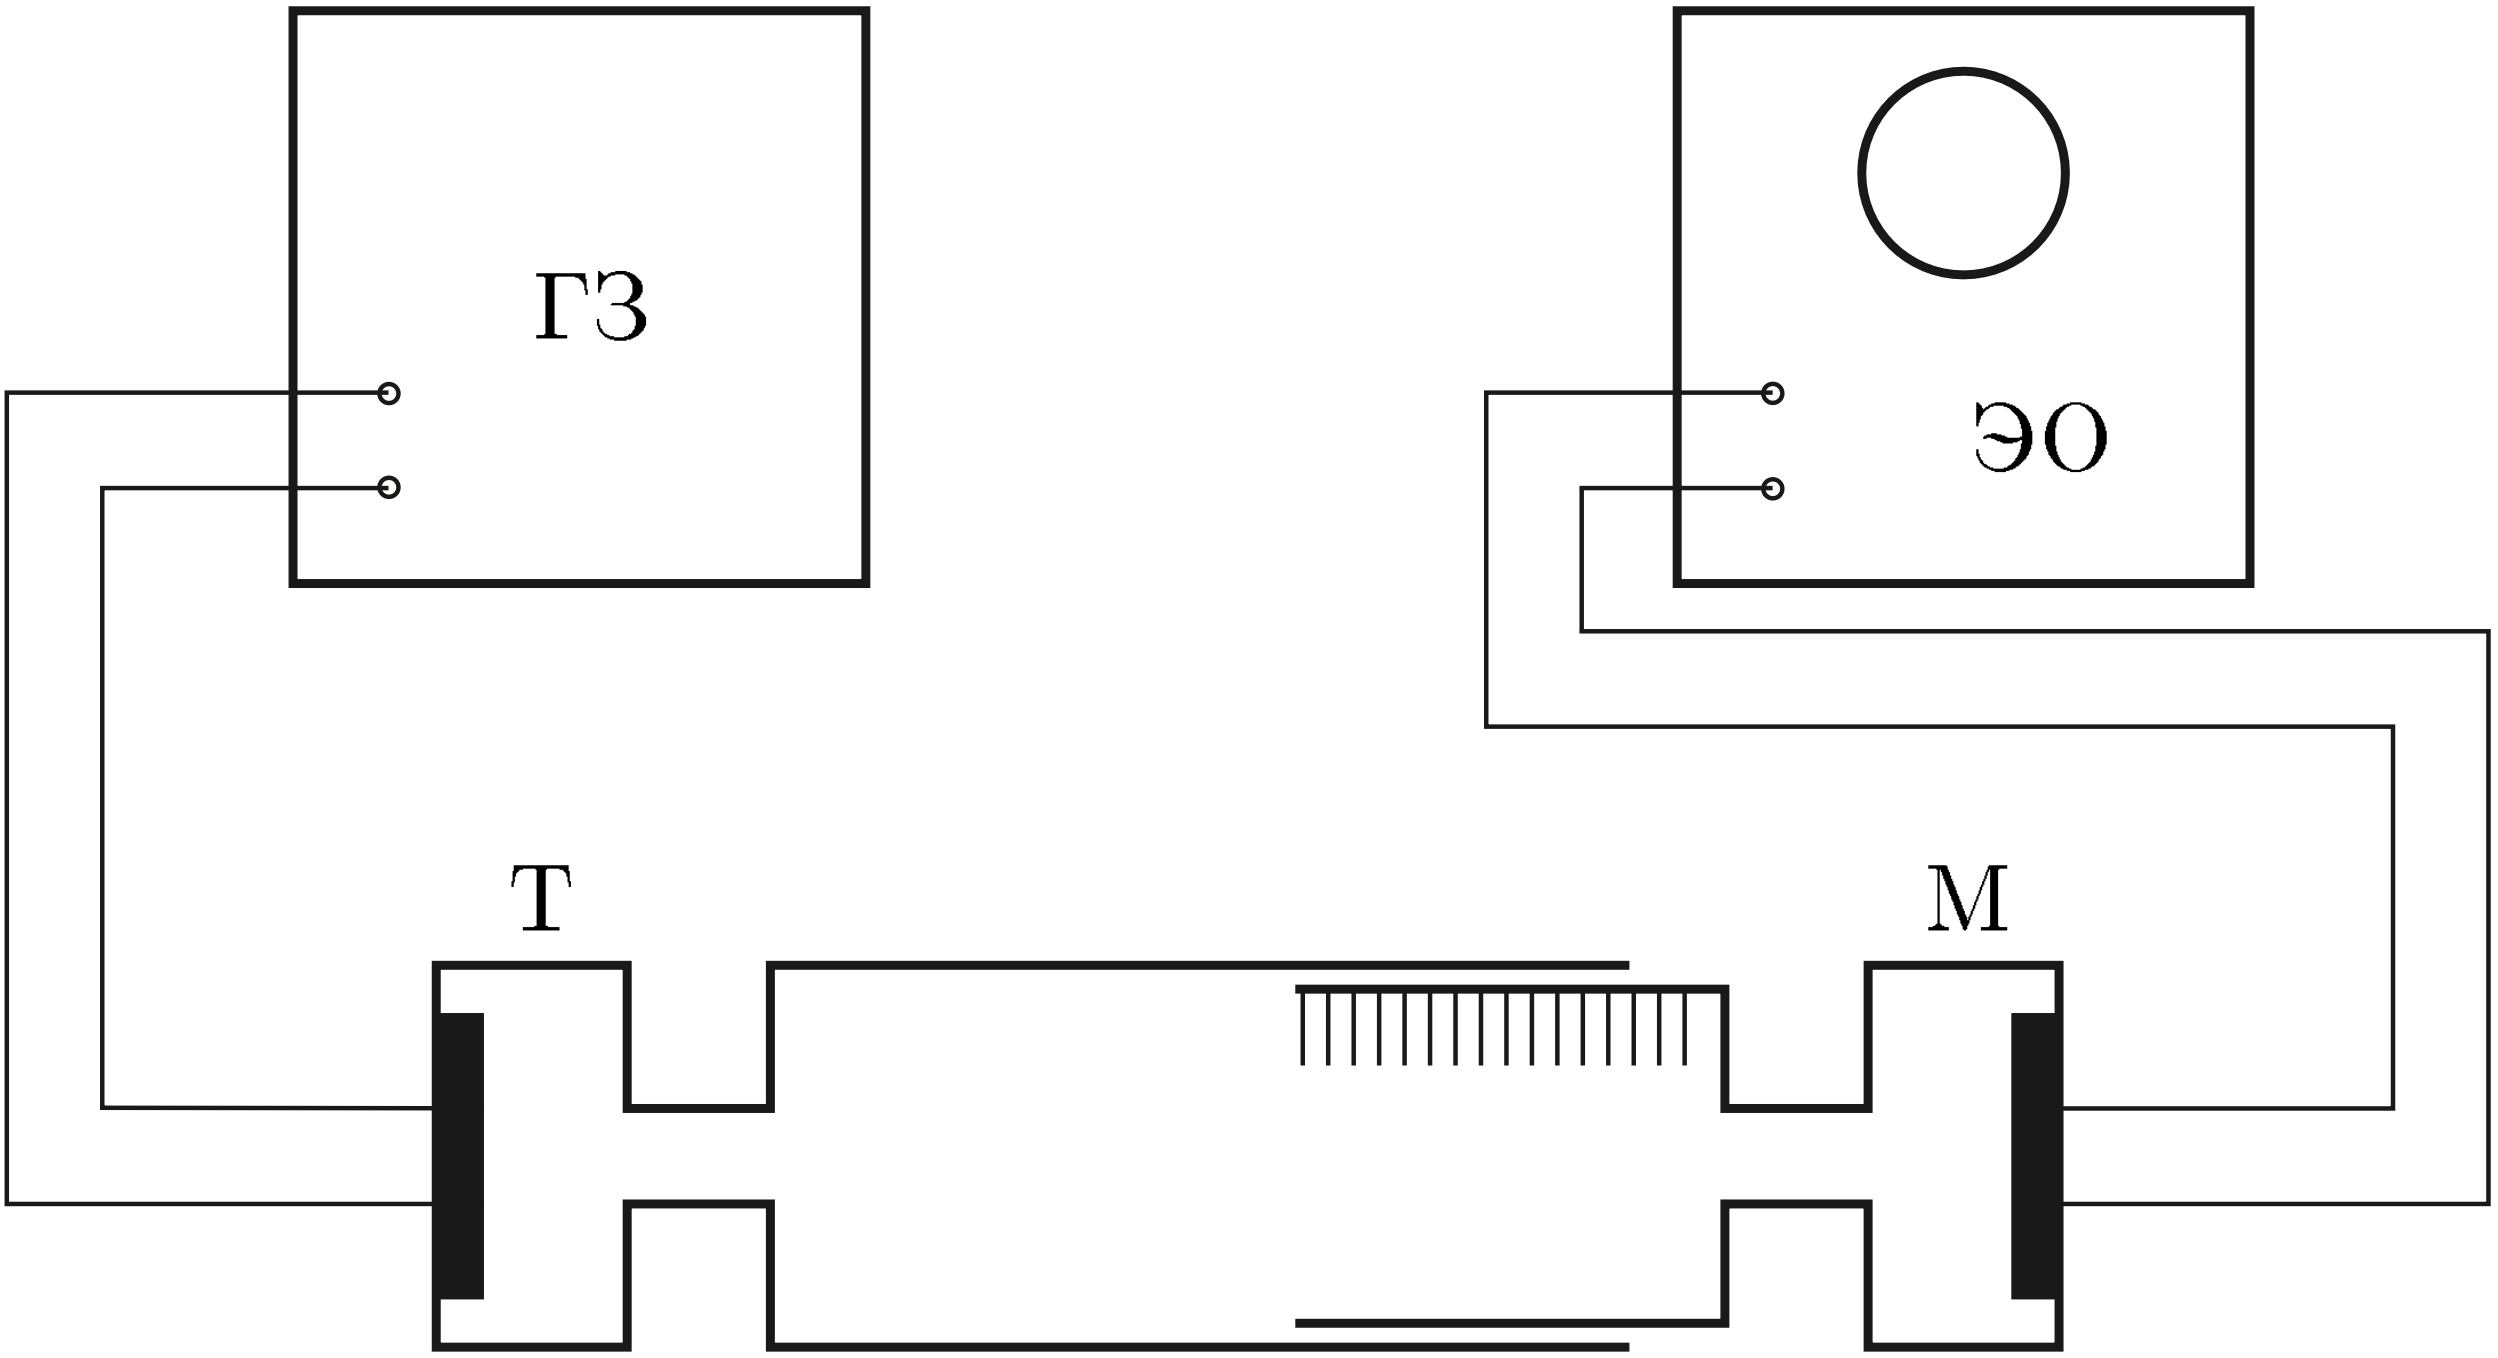
\includegraphics[width=\textwidth]{установка1.png}
    \caption{Установка для измерения скорости звука при помощи раздвижной трубы}\label{setup}
	\label{setup1}
\end{figure}

\begin{figure}[h!]
    \centering
    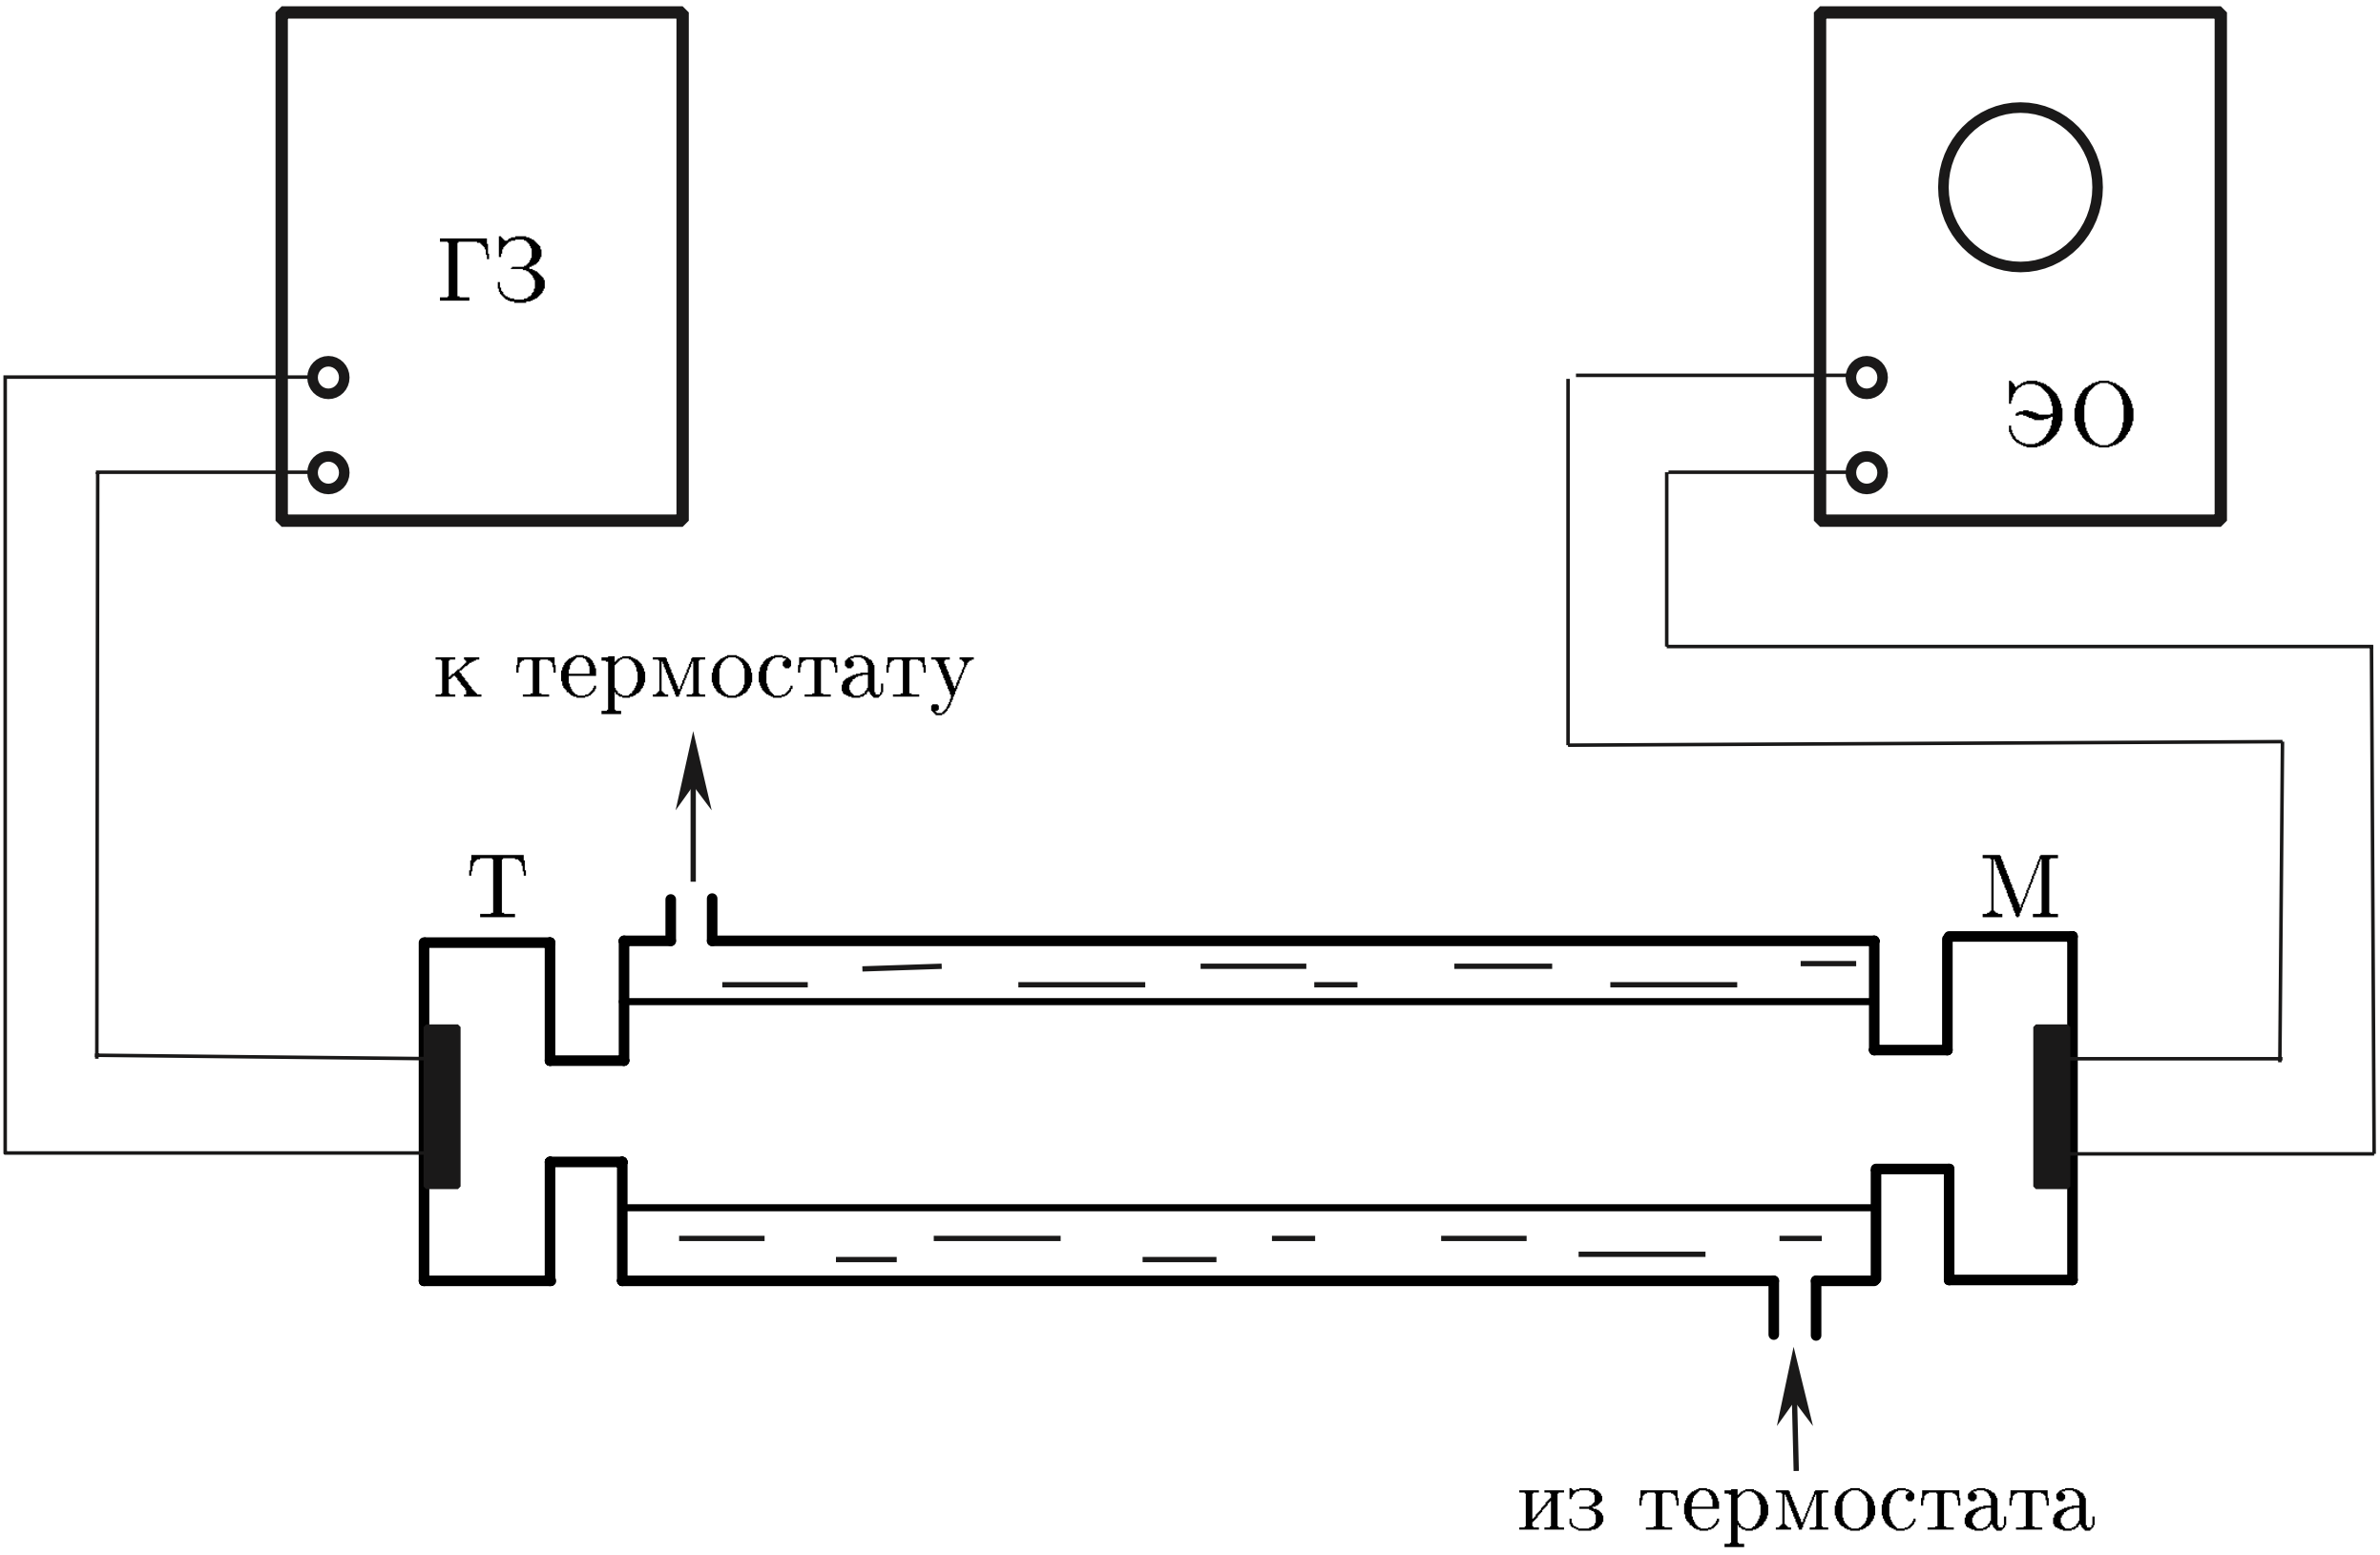
\includegraphics[width=\textwidth]{установка2.png}
    \caption{Установка для изучения зависимости скорости звука от температуры}\label{setup}
	\label{setup2}
\end{figure}

% \section{Методика измерений}
\clearpage
\newpage
% \mbox{~}
% \clearpage
% \newpage

\section{Результаты измерений и обработка данных}

Используя коэффициент наклона каждой из прямых, найдем зависимость скорости от темепературы по формуле (\ref{5}):

\begin{figure}[h!]
    \centering
    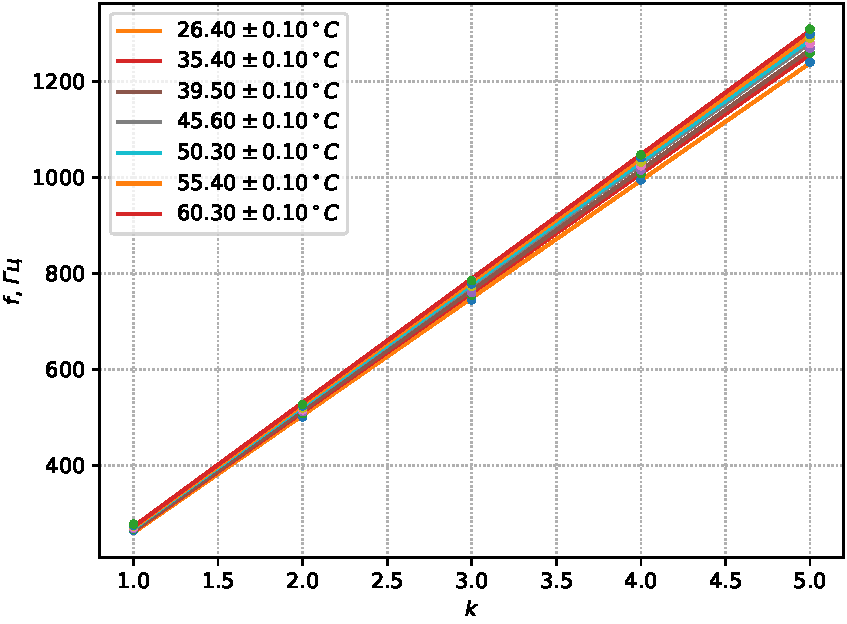
\includegraphics[width=0.77\textwidth]{f.pdf}
    \caption{Зависимость частоты от номера резонанса для разных температур}
	% \label{setup1}
\end{figure}

Постороим зависимость квадрата скорости от темепературы:

\begin{figure}[h!]
    \centering
    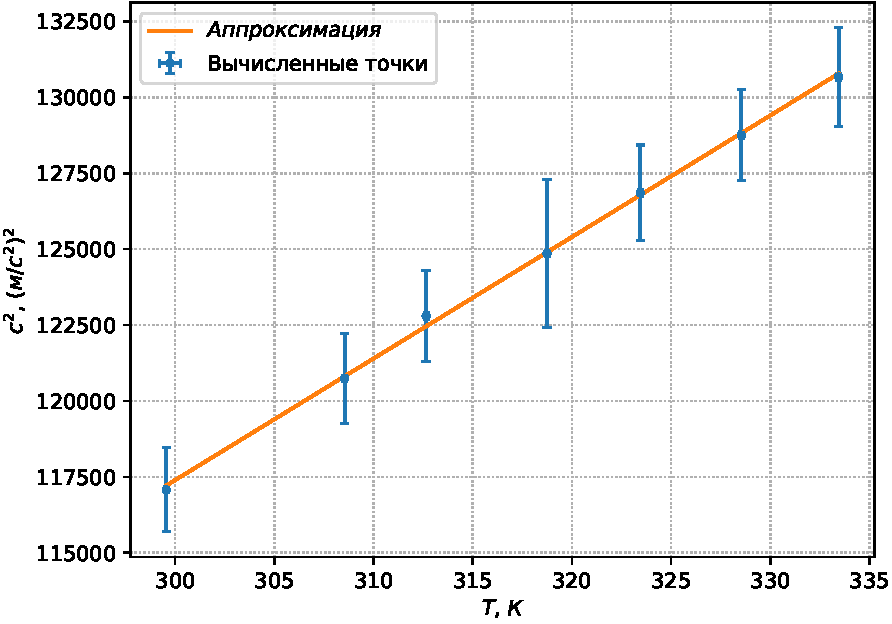
\includegraphics[width=0.77\textwidth]{c.pdf}
    \caption{Зависимость частоты от температуры при постоянной длине трубки}
	% \label{setup1}
\end{figure}

Используя коэффициент наклона последнего графика, найдем показатель адиабаты по формуле (\ref{gamma}):
\begin{equation}
	\gamma=1.394 \pm 0.022

\end{equation}


% \section{Обсуждение результатов}

\end{document}
